% Chapter Template

\chapter{Results - Sliding Puzzle} % Main chapter title

\label{sec:ResultsSP} % Change X to a consecutive number; for referencing this chapter elsewhere, use \ref{ChapterX}

%----------------------------------------------------------------------------------------
%	SECTION 1
%----------------------------------------------------------------------------------------

\section{Low dimension}
\label{sec:SPLowDimension}

As mentioned in chapter \ref{sec:Puzzles}, the state space cardinality for the SP grows very quickly with n and m. Here are the only dimensions which have less than 239.5 millions states. Note I am also only considering n $\leq$ m since (p, q) can always be solved if we know how to solve (q, p):
\\
\\
\begin{center}
\begin{tabular}{l*{6}{c}r}
n              & m & 2 & 3 & 4 & 5\\
\hline
2              &   & 12 & 360 & 20,160 & 1,814,400 \\
3              &   &   & 181,440 &  &    \\
\end{tabular}
\end{center}
In this section, I will discuss \textbf{full} results for these 5 puzzles. In order to fully solve them, one can simply use rubiks.scripts.learner, setting up the PerfectLearner with A* and manhattan heuristic, or instantiate directly a PerfectLearner as have seen in section \ref{PLSS}
I obtained the following God numbers for these puzzles:
\begin{center}
\begin{tabular}{l*{6}{c}r}
n              & m & 2 & 3 & 4 & 5\\
\hline
2              &   & 6 & 21 & 36 &  \\
3              &   &   & 31 &  &    \\
\end{tabular}
\end{center}
and the most difficult puzzles (requiring a number of steps equal to their respective God number to solves):
\\
\\
\underline{Most difficult 2x2 (6 moves)}:
\begin{center}
\begin{three}
\setrow{2}{,3}
\setrow{1}{2,1}
\end{three}
\end{center}
\underline{Most difficult 2x3 (21 moves)}:
\begin{center}
\begin{five}
\setrow{2}{4,5,}
\setrow{1}{1,2,3}
\end{five}
\end{center}
\underline{Most difficult 2x4 (36 moves)}:
\begin{center}
\begin{seven}
\setrow{2}{,7,2,1}
\setrow{1}{4,3,6,5}
\end{seven}
\end{center}
\underline{Most difficult 2x5 (47 moves) .... TBD }:
\begin{center}
\begin{nine}
\setrow{2}{,2,7,4,1}
\setrow{1}{5,8,3,9,6}
\end{nine}
\end{center}
\underline{Most difficult 3x3 (31 moves)}:
\begin{center}
\begin{eight}
\setrow{3}{8,6,7}
\setrow{2}{2,5,4}
\setrow{1}{3,,1}
\end{eight}
\end{center}



%-----------------------------------
%	SECTION 2
%-----------------------------------
\section{Intermediary case - 3x3}
\label{S33}


\subsection{Perfect learner}
As seen in the previous section section \ref{sec:SPLowDimension}, the 3 by 3 SP is one of the cases we have been able to solve perfectly, since it only has 181,440 possible configurations. Its God number is only 31, which definitely makes it manageable. However, this is already an intermediary size, large enough to make trying deep reinforcement learning meaningful. The PerfectLearner's learning are shown in figure \ref{fig:33SPPerfectLearning}:


\newgeometry{top=0mm, bottom=0mm, left=0mm, right=0mm}
\begin{landscape}
\centering\vspace*{\fill}
\begin{figure}[H]
\centering
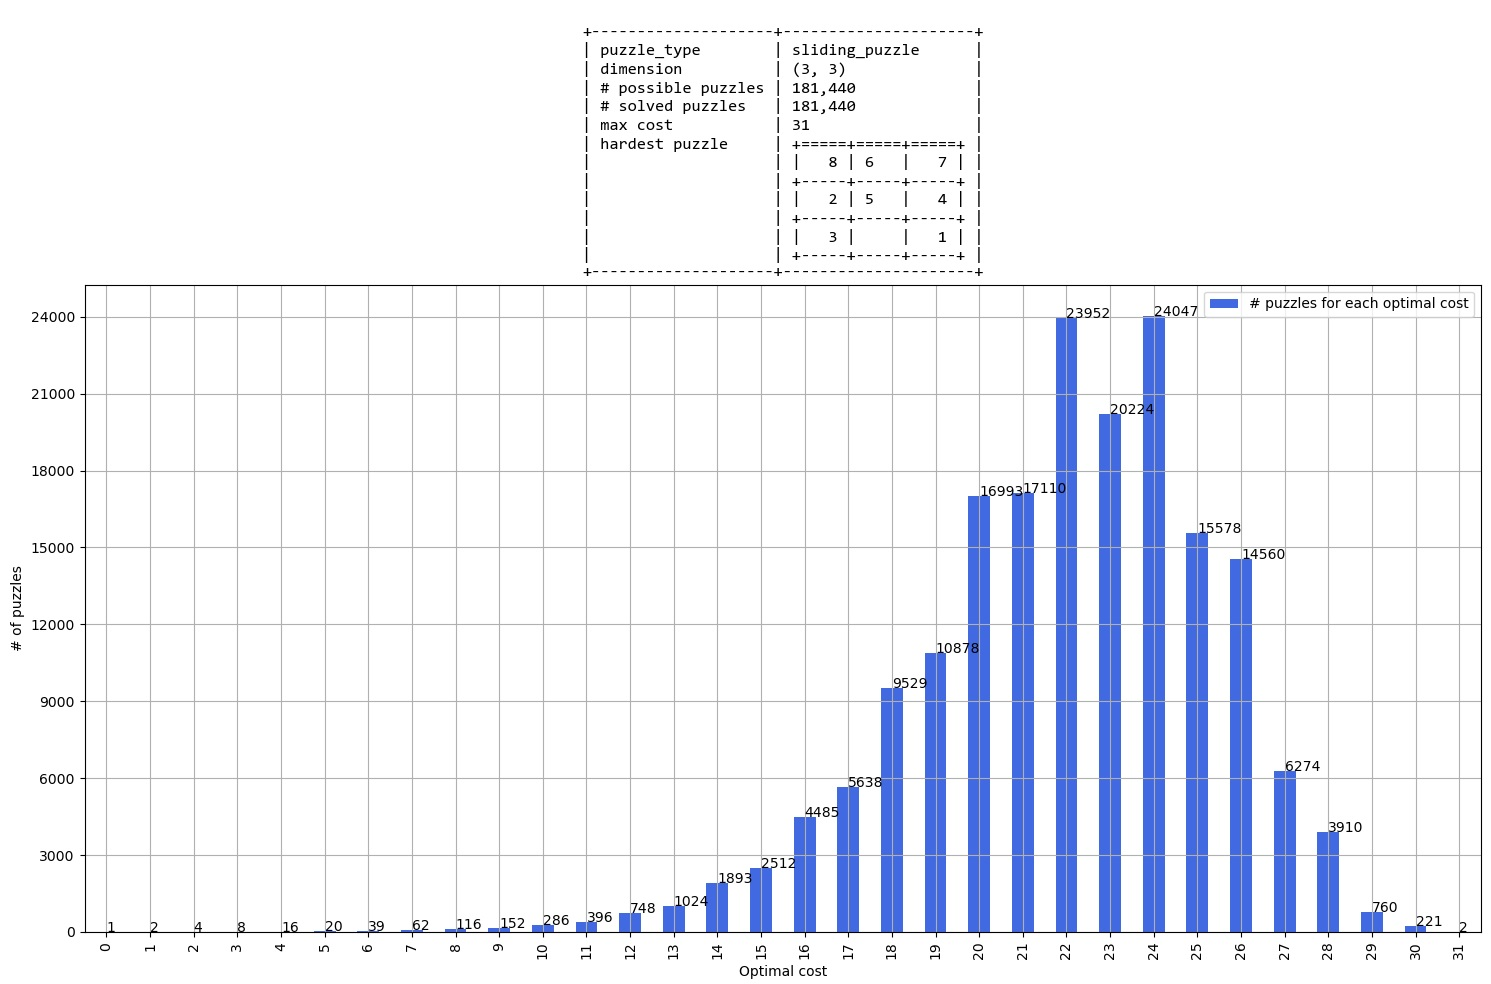
\includegraphics[scale=0.7]{./Figures/33SPPerfectLearning.jpeg}
%\decoRule
\caption[33SPPerfectLearning]{Perfect Learning 3x3 SP}
\label{fig:33SPPerfectLearning}
\end{figure}
\vfill
\end{landscape}
\restoregeometry




\subsection{Deep reinforcement learner}
 The DeepReinforcementLearner's learning is shown in figure \ref{fig:33SPDeepReinforcementLearning}:

\newgeometry{top=0mm, bottom=0mm, left=0mm, right=0mm}
\begin{landscape}
\centering\vspace*{\fill}
\begin{figure}[H]
\centering
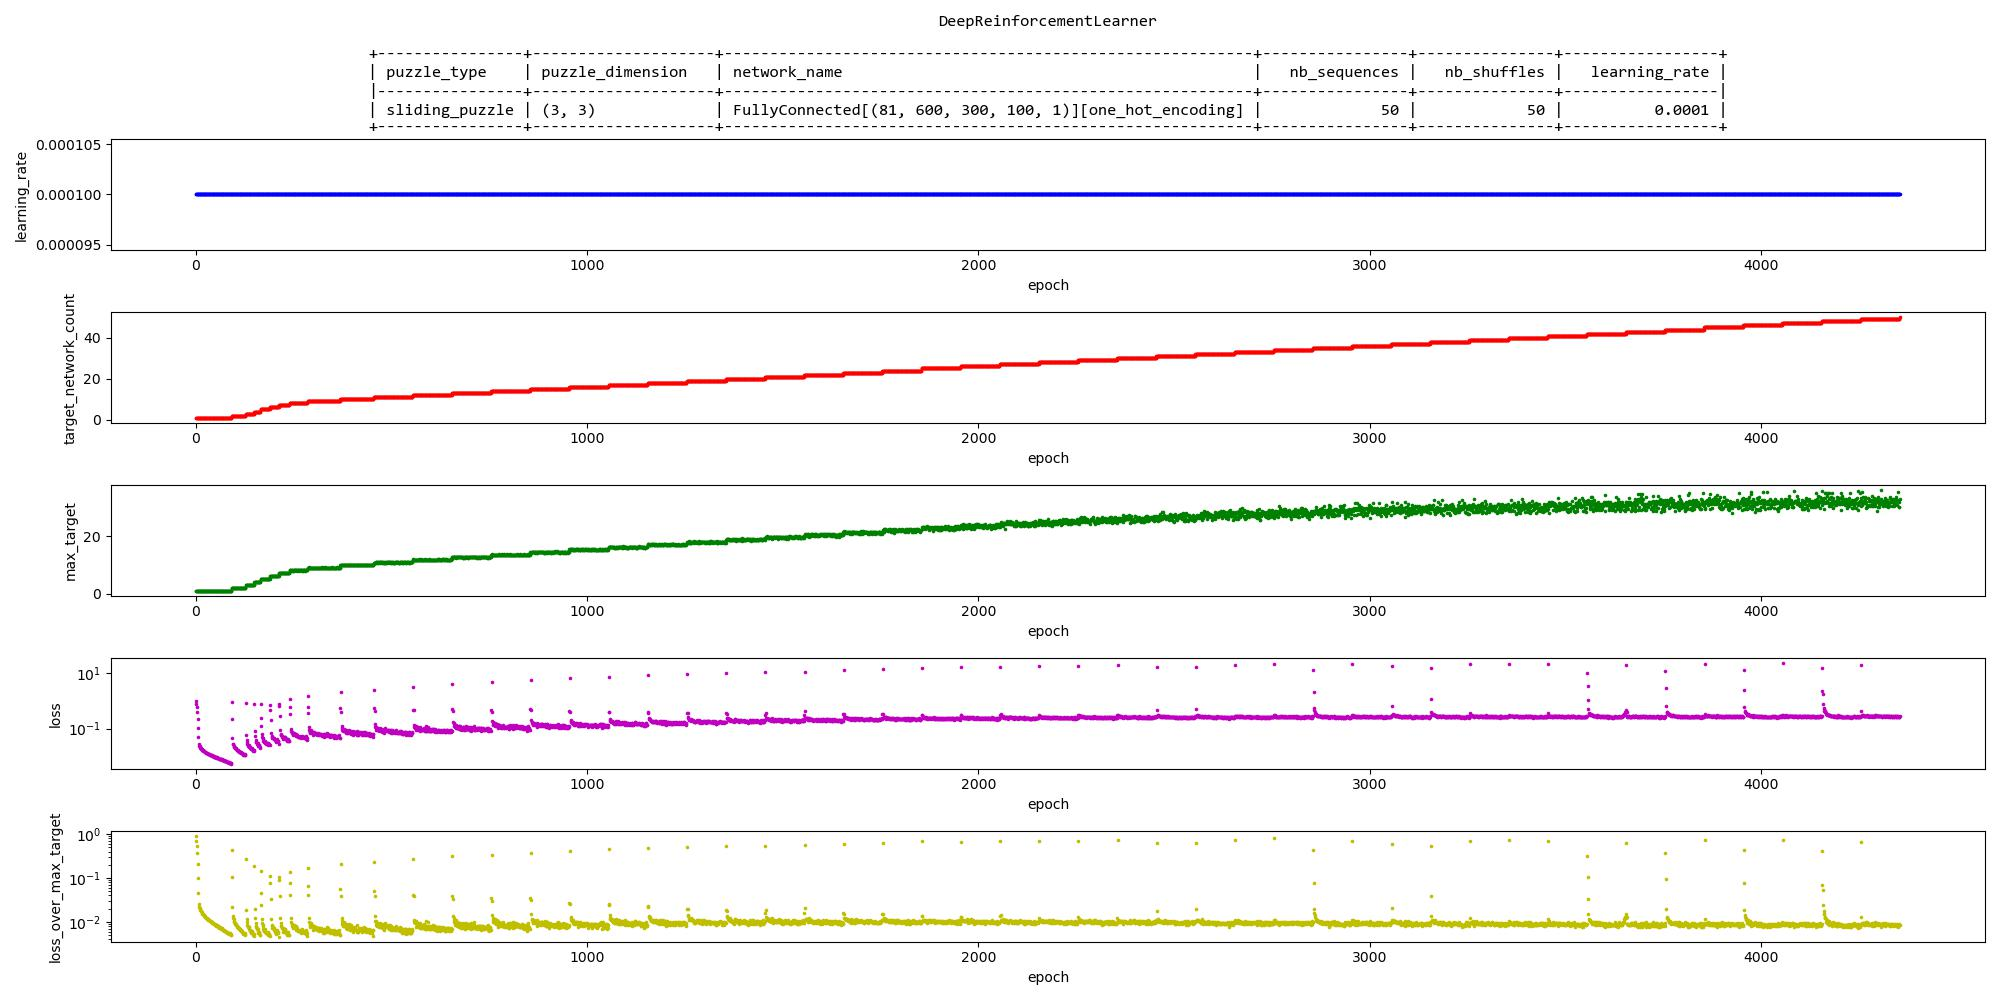
\includegraphics[align=c, scale=0.55]{./Figures/33SPDeepReinforcementLearning.jpeg}
\caption[33SPDeepReinforcementLearning]{Deep reinforcement learner 3x3 SP}
\label{fig:33SPDeepReinforcementLearning}
\end{figure}
\vfill
\end{landscape}
\restoregeometry


\subsection{Solvers' comparison}
Finally, to conclude this section on the 3x3 case, let's us discuss a comparison of several algorithms on 1000 random puzzles generated for a number of random shuffling (with best effort no backtracking) from 0 to 50 in step of 2, as well as for perfect shuffling (denoted by $\infty$) on the comparison graphs. The results are shown in figure \ref{fig:33SPPerformance}

\newgeometry{top=0mm, bottom=0mm, left=0mm, right=0mm}
\begin{landscape}
\centering\vspace*{\fill}
\begin{figure}[H]
\centering
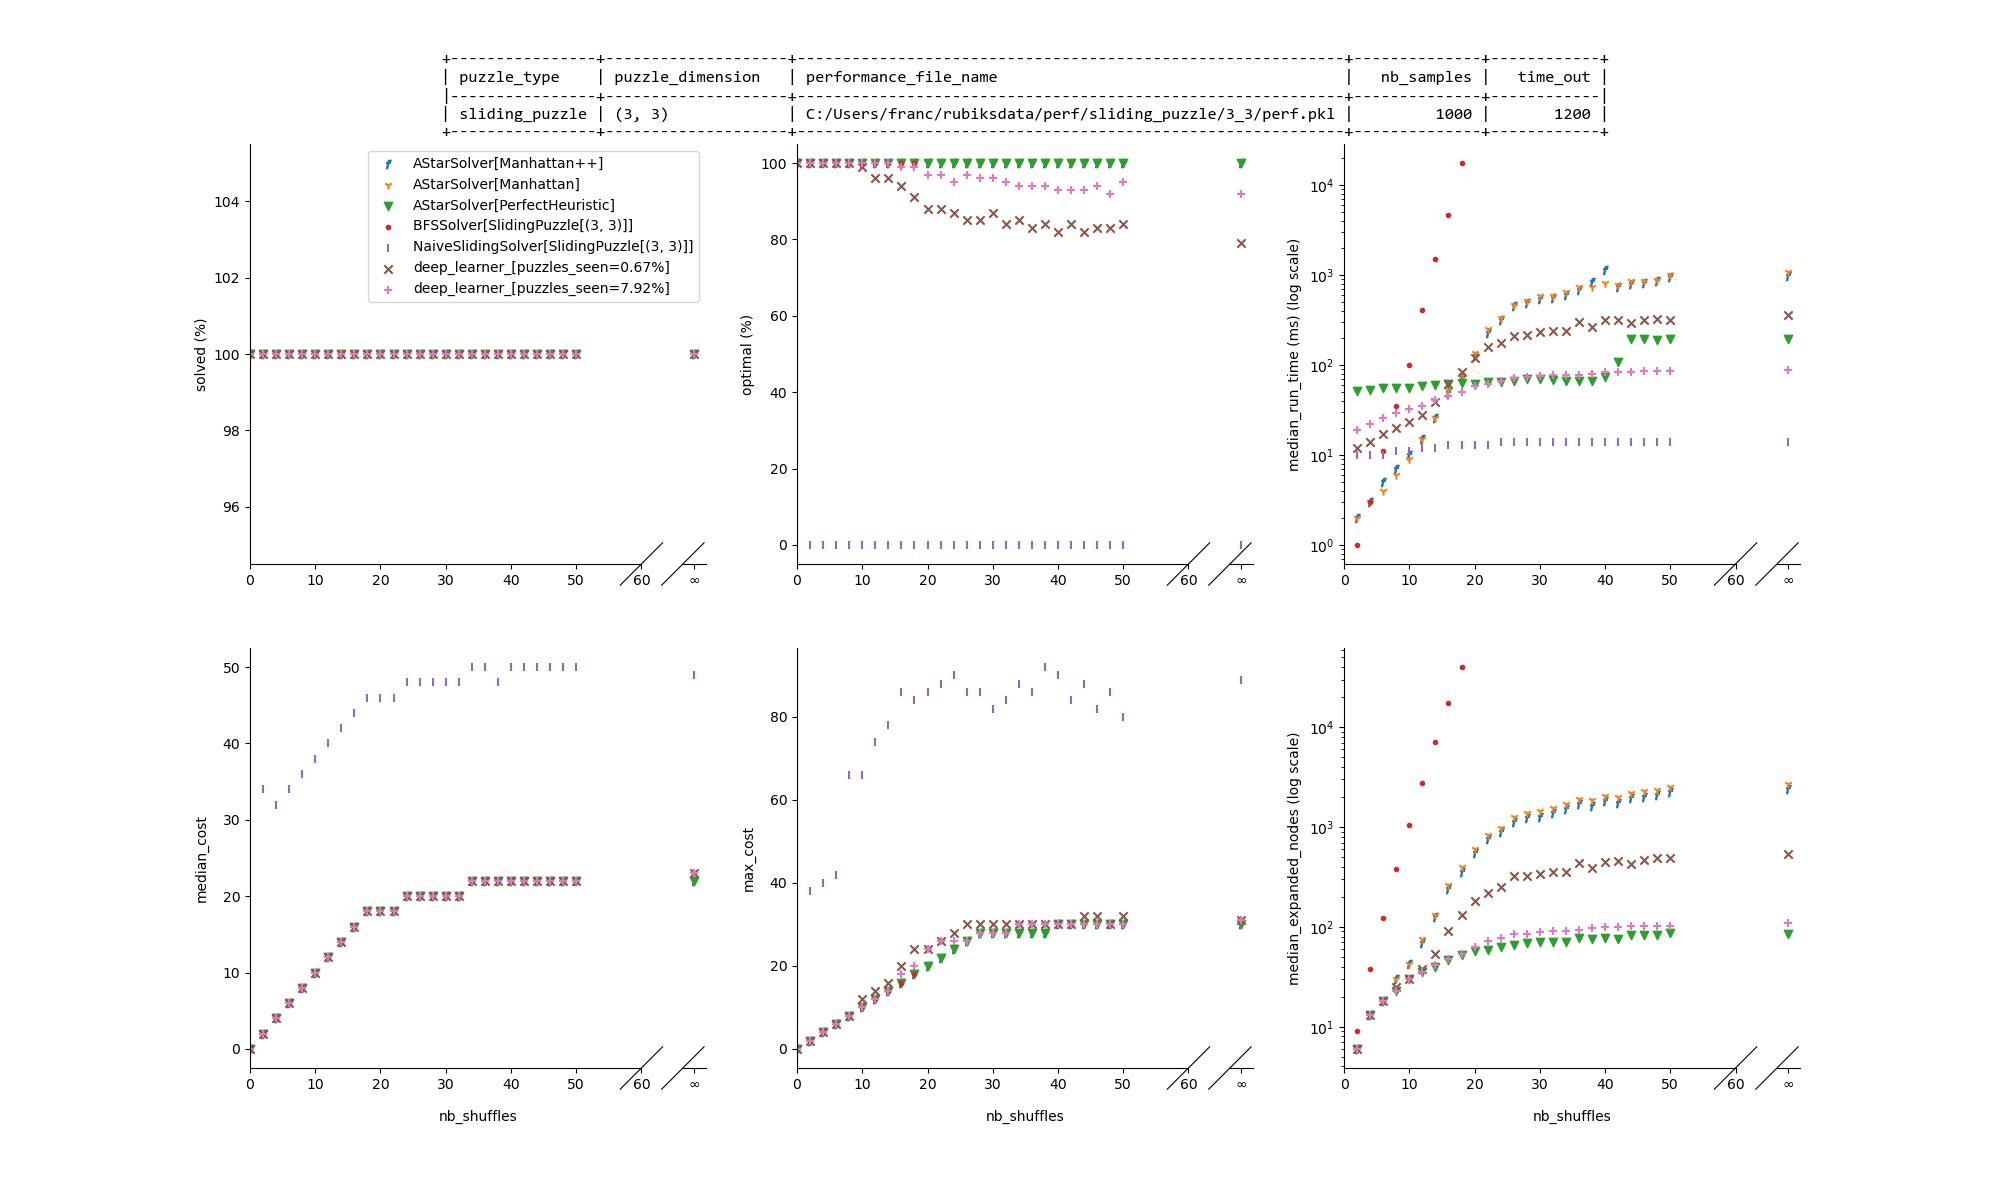
\includegraphics[scale=0.63]{./Figures/33SPPerformance.jpeg}
%\decoRule
\caption[33SPPerformance]{Solvers' performance comparison 3x3 SP}
\label{fig:33SPPerformance}
\end{figure}
\vfill
\end{landscape}
\restoregeometry


%-----------------------------------
%	SECTION 3
%-----------------------------------
\section{3x4}

blabla

%-----------------------------------
%	SECTION 4
%-----------------------------------

\section{4x4}

blabla
